\documentclass[11pt,fleqn]{article} % Default font size and left-justified equations

%\usepackage{standalone}

\usepackage{comment}
\begin{comment}
Modification History:
  180803 David Shifflett
    Fixed 'git clone https' syntax, added 'git clone git@' example
\end{comment}

\usepackage{todonotes}
\usepackage{color}
\usepackage{paralist}
% use \todo{note} OR \missingfigure{Add my picture here}

\include{structure}

\setcounter{secnumdepth}{5}
\setcounter{tocdepth}{5}

%\usepackage{arabtex}

\usepackage{verbatim}

\raggedbottom

\begin{document}

%define macros for commonly used terms that require special formatting
\newcommand \mpgt {\textit{MP Gryphon Toolset}\xspace}
\newcommand \ggui {\textit{MP Gryphon GUI}\xspace}
\newcommand \gtg {\textit{MP Gryphon Trace Generator}\xspace}
\newcommand \mphoenix {\textit{Monterey Phoenix}\xspace}

\hypersetup{%
    pdfborder = {0 0 0}
}

\lstdefinestyle{customfile}{
basicstyle=\footnotesize\ttfamily, frame=single, float=htpb}

\input{./title.tex}

\pagenumbering{roman}
\setlength{\parindent}{0pt} %remove indenting from whole document
\newpage
\thispagestyle{empty}
\mbox{}
\newpage

\tableofcontents
\newpage
\pagenumbering{arabic}
\newpage

\section{Introduction}
\label{intro}
\subsection {Overview}
The \mpgt supports \mphoenix users with tools for building MP Code and generating trace graphs calculated from MP code.
The \mpgt consists of the \ggui and the \gtg:\\
\begin{compactitem}
\item The \ggui tool is the graphical interface tool for editing MP Code and for running the \gtg engine to view generated traces.
\item The \gtg tool compiles MP Code into traces that the \ggui can read and graph.\\
\end{compactitem}

\subsection{Compatibility}
\ggui Version 0.3.0 is compatible with \mphoenix Version 4 pre-alpha and \gtg Version 4 pre-alpha.
% \ggui Version 0.3.0 is expected to be compatible with future versions of \mphoenix Version 4.

\section{Installing the \mpgt}
You will need the \ggui and the \gtg.
%  What you need depends on whether you are running Mac/Linux or Windows and the installation approach you choose.
For now, for Mac/Linux: clone \mpgt source code directly from their Git repositories by typing the following:
\begin{Verbatim}[commandchars=\\\{\}]
\verbbf{git clone https://gitlab.nps.edu/monterey-phoenix/user-interfaces/MP_Gryphon_GUI.git}
\verbbf{git clone https://gitlab.nps.edu/monterey-phoenix/trace-generator.git}
\end{Verbatim}

or
\begin{Verbatim}[commandchars=\\\{\}]
\verbbf{git clone git@gitlab.nps.edu:monterey-phoenix/user-interfaces/MP_Gryphon_GUI.git}
\verbbf{git clone git@gitlab.nps.edu:monterey-phoenix/trace-generator.git}
\end{Verbatim}

To clone from GitLab you will need to upload your public RSA Key as described at \url{https://gitlab.nps.edu/help/ssh/README.md}.\\

\subsection{Installing Python 3}
Install Python3 if it is not already present. To see if Python3 is already installed, you may type the following at a command prompt and verify that Python Version 3 is present:
\begin{compactitem}
%\item Windows:
%\begin{Verbatim}[commandchars=\\\{\}]
%\verbbf{python --version}
%\end{Verbatim}
\item Mac/Linux:
\begin{Verbatim}[commandchars=\\\{\}]
\verbbf{python3 --version}
\end{Verbatim}
\end{compactitem}
If not already present, you may download and install Python3 for your system from \url{https://www.python.org/download/releases/3.0}.\\
%If installing on Windows, you must check the ``Add Python to PATH'' checkbox when installing Python or you will get an error indicating that Python is not recognized.\\

Linux users may prefer to install Python 3 using their package manager, for example Fedora users might type:
\begin{Verbatim}[commandchars=\\\{\}]
\verbbf{sudo dnf install python3+}
\end{Verbatim}

\subsection{Installing PyQt5}
The \ggui requires PyQt5.
Please type the following at a command prompt to install PyQt5:
\begin{compactitem}
%\item Windows:
%\begin{Verbatim}[commandchars=\\\{\}]
%\verbbf{python -m pip install PyQt5}
%\end{Verbatim}
\item Mac/Linux:
\begin{Verbatim}[commandchars=\\\{\}]
\verbbf{python3 -m pip install PyQt5}
\end{Verbatim}
\end{compactitem}

\subsection{Building the \gtg}
If you installed on Linux using the repositories then the \gtg must be built.
First, please install requisites needed for running \verb+make+.
Mac users may be asked to install Command line developer tools, which are required.  Linux users need to install 32-bit CLib and the csh shell. Syntax depends on Linux flavor.  A Fedora dnf example is to type:
\begin{Verbatim}[commandchars=\\\{\}]
\verbbf{sudo dnf install glibc-devel.i686}
\verbbf{sudo dnf install tcsh.x86_64}
\end{Verbatim}

An Ubuntu apt example is:
\begin{Verbatim}[commandchars=\\\{\}]
\verbbf{sudo apt install libc6-dev-i386}
\verbbf{sudo apt install csh}
\end{Verbatim}

Build the trace generator engine from a command window by navigating to the \verb+MP_Gryphon_Trace_Generator/RIGAL/src+ directory and typing:
\begin{Verbatim}[commandchars=\\\{\}]
\verbbf{make}
\end{Verbatim}

%%% For zip or Windows installer:
%\subsubsection{Downloading and Running the \ggui}
%\begin{compactitem}
%\item Windows users:
%  \begin{compactenum}
%  \item Download the \ggui Windows Installer from the \mpgt Download page.
%  \item Click on the download and run the installer.
%  \item Start the \ggui tool by clicking on the \ggui tool icon.
%  \end{compactenum}
%\item Mac, Linux flavors, and Windows users: All users may install and run the \ggui \verb+.zip+ distribution as follows:
%  \begin{compactenum}
%  \item Download the \ggui \verb+.zip+ distribution from the \mpgt Download page.  For example you might download it to\\
%\verb+/Users/<yourname>/Downloads+.
%  \item Unzip the distribution.
%  \item From a command window, navigate to the \verb+MP_Gryphon_GUI/python/+ subdirectory, for example to path\\
%\verb+/Users/<yourname>/Downloads/MP_Gryphon_GUI_<latest version>/python+ and type:
%\begin{Verbatim}[commandchars=\\\{\}]
%\verbbf{./mp.py}
%\end{Verbatim}
%  \end{compactenum}
%\end{compactitem}
%

\section{Launching the \ggui}
For Linux users: from a command window, navigate to the \verb+MP_Gryphon_GUI/python/+ subdirectory, for example to path\\
\verb+/Users/<yourname>/Downloads/MP_Gryphon_GUI_<latest version>/python+ and type:
\begin{Verbatim}[commandchars=\\\{\}]
\verbbf{./mp.py}
\end{Verbatim}

\subsection{Configuring the \ggui}
Once launched, the \ggui may be configured using its menu controls under \verb+Preferences+:
\begin{compactitem}
\item Several graph appearance options are available optimized for brightness, printing, a classic look, etc.\\
\end{compactitem}


\section{Working with the \ggui}
To write your own system models, a working knowledge of \mphoenix technology and MP Code syntax is required. Please visit \url{https://wiki.nps.edu/display/MP/Monterey+Phoenix+Home} for information about working with \mphoenix technology.

\section{\ggui User Interfaces}
%\subsection{Main Window}
This section describes user interfaces available to \ggui.
Here is an example screenshot of the \ggui main window:\\
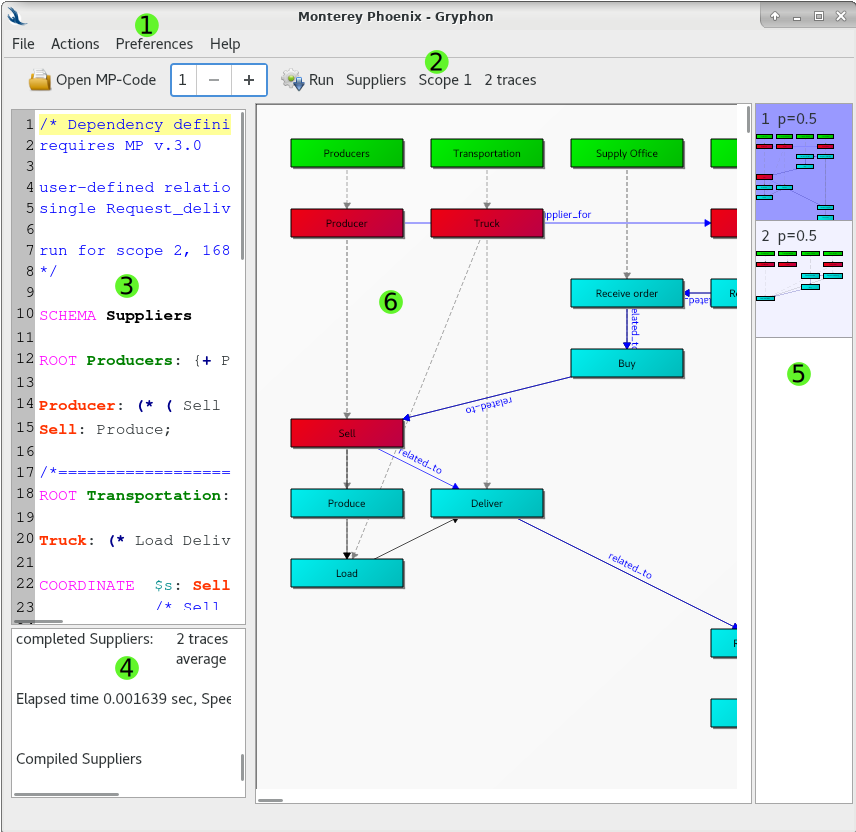
\includegraphics[scale=.65]{screenshots/main_window_sectioned}\\
The following parts are shown:
\begin{compactenum}
\item Menu controls
\item Trace generator controls and status
\item MP Code editor pane
\item Log pane
\item Trace selection list
\item Main trace view pane
\end{compactenum}

\subsection{Menu Controls}
Menu controls include:
\begin{compactitem}
\item \textbf{File}
  \begin{compactitem}
  \item Open, save MP Code, open examples.
  \item Import and export projects.
  \item Export one or all traces.
  \end{compactitem}
\item \textbf{Actions}
  \begin{compactitem}
  \item Run the trace generator engine.
  \item Clear the Log pane.
  \end{compactitem}
\item \textbf{Preferences}
  \begin{compactitem}
  \item Graph Settings: Set graph settings:
    \begin{compactitem}
    \item Bright - View with high color contrast.
    \item Print - View with colors that are more readable when printed.
    \item Classic - Use classic Firebird coloring.
    \item Custom - Set, save, share your own color scheme.
    \end{compactitem}
  \item Server: Set to connect to a \gtg Server or to use the \gtg locally.
  \end{compactitem}
\item \textbf{Help}
  \begin{compactitem}
  \item View help for the \mpgt.
  \item View information about \mpgt.
  \end{compactitem}
\end{compactitem}

\subsection{Trace generator controls and status}
Trace generater controls and status are available in the toolbar, for example:\\
\includegraphics[scale=.4]{screenshots/toolbar}.\\
Hover the cursor over controls to see tooltips. Controls include:
\begin{compactitem}
\item The ``Open MP Code File'' button (\includegraphics[scale=.4]{screenshots/open_mp_code_file}) for opening a MP Code file.
\item The ``Scope'' selector
(\includegraphics[scale=.4]{screenshots/scope_spinner})
for selecting the scope for trace generation.
\item The ``Run'' button (\includegraphics[scale=.4]{screenshots/run})
for running the trace generator engine on the MP Code.
\end{compactitem}
Status describes information about the currently loaded trace generation view.
In this example,
\includegraphics[scale=.4]{screenshots/example_status}:
\begin{compactitem}
\item \verb+Suppliers+ is the name of the schema as defined in the MP Code.
\item \verb+Scope 1+ indicates that the trace generator engine was run for the MP Code at scope level 1.
\item \verb+2 traces+ indicates that the trace generator engine produced two traces.
\end{compactitem}

\subsection{MP Code Editor Pane}
Manage MP Code using the MP Code editor pane:
\begin{compactitem}
\item Open, import, paste, or edit your MP Code.
\item Syntax highlighting identifies keywords, root events, composite events, etc.
\item Run the trace generator engine (\includegraphics[scale=.4]{screenshots/run}) at the desired scope to generate traces from your MP Code.
\end{compactitem}

\subsection{Log Pane}
The log pane provides a log of actions taken and of trace generator output. It is available for reference. You may clear it using menu control \verb+File | Actions | Clear MP Code Log+.

\subsection{Trace selection list}
The trace selection list contains a list of all possible traces given your MP Code and scope.
At the top of each trace is its trace index and the probability of that trace occurring. The sum of probabilities across all traces is 1.0.

\begin{compactitem}
\item Scroll down the trace list to view all traces.
\item Click on a trace to select it in the main trace view pane.
\end{compactitem}

\subsection{Main Trace View Pane}
The Main trace view pane contains the currently selected trace.
You may adjust this view as follows:
\begin{compactitem}
\item Pan by dragging the mouse or moving the scrollbars.
\item Zoom by moving the mouse wheel or by pressing the \verb.+. or \verb+-+ keys. The zoom focal point is at the cursor.
\item Drag nodes to move them.
\item You may also adjust view settings using menu control \verb+Preferences | Graph Settings | Custom...+.
\item Future work:
  \begin{compactitem}
  \item Nodes will have menus for collapse, expand, etc.
  \item Edges may be movable.
  \end{compactitem}
\end{compactitem}

\subsection{Keyboard Shortcuts}
\subsubsection{Graph Window Shortcuts}
\begin{compactitem}
\item CTRL + Click on event (Command + Click on Mac): Toggle select or unselect individual events.
\item SHIFT + Click on event: Select event and all events below it bound by IN relation.
\item Click empty space: Unselect all events.
\item Click on empty space and drag: Pan the view.
\item SHIFT + Click empty space and drag: Select events in range.
\item CTRL + A (Command + A on Mac): Select all events.
\item Keyboard arrow keys: Pan the view.
\item + and - keys: Zoom in and out.
\item Click menu tab: Open menu for an event.
\item Right-click event: Open menu for an event.
\item H: Toggle hide/unhide selected event(s).
\item C: Toggle collapse/uncollapse selected Root and Composite event(s). Results may be unexpected if multiple events are selected.
\end{compactitem}

\subsubsection{Code Window Shortcuts}
\begin{compactitem}
\item Click word to highlight word.
\item Click or Navigate to parenthesis to find its mate.
\item CTRL + Spacebar or type first three letters: Show auto-complete hints for existing events or keywords.
\end{compactitem}

\subsubsection{Graph List Shortcuts}
\begin{compactitem}
\item Up and down arrows: Select previous or next trace.
\end{compactitem}

\section{Examples}
Please obtain, install, and start the \ggui graphical interface per installation instructions, above.
\subsection{Load and run MP Code Example 1}
In this example we open and run MP Code example 1 at Scope 2, select and adjust trace 2, and save the view as a \verb+.png+ image file.

\begin{compactenum}
\item Under menu control \verb+File | Open MP Code Example+ select example\\
\verb+Example_1_simple_message_flow.mp+.
The MP Code listing will show up in the code editor pane.
\item Set the scope to 2 by adjusting the Scope spinner trace generator control.
\item Run the trace generator engine by pressing the run icon
(\includegraphics[scale=.4]{screenshots/run}).
Three traces will be generated. All three traces will be visble in the trace selection list. The first trace will be visible in the main trace view pane.
\item Select the third trace in the list. This trace will be drawn in the main trace view.
\item Move some nodes as desired by dragging them with the cursor.
\item Export the third trace to a \verb+.png+ file using menu \verb+File | Export Trace...+.
\item If you would like to print your exported traces, you may wish to select menu control \verb+Preferences | Graph Settings | Contrast+ for higher contrast for printing before exporting them. Or select menu control \verb+Preferences | Graph Settings | Custom...+ to configure your own graph view scheme.
\end{compactenum}

\section{Reporting Bugs}
Please report any bugs encountered during operation of the \mpgt.  To assist in diagnosing your bug, please include the following informtion:
\begin{compactitem}
\item The \verb+.mp+ code, Scope number, and selected Trace used when the error occurred.
\item The steps taken that can be used to recreate the error.
\item The version of the \ggui tool used.
\item The Operating System you used.
\end{compactitem}

\section{Post-processing Analysis}
The \ggui tool exports graph data in JSON Graph format (JGF).
This output may be used during post-processing analysis of graph data or for input to third party tools which can accept JGF data as input.
The JGF standard defines names for \verb+graph+, \verb+node+, and \verb+edge+ fields. The \ggui tool extends these fields by including additional information such as graph positioning, the trace \verb+mark+ field, Cubic Bezier edge points for curved edges, and whether nodes are hidden or collapsed.
For more information on JGF please see \url{http://jsongraphformat.info}. For syntax of JSON data exported by the \ggui tool, please use the export command to create your own JSON \verb+.gry+ file and use that as a reference.

\end{document}
